\documentclass[conference]{IEEEtran}
\usepackage{cite}
\usepackage{amsmath,amssymb,amsfonts}
\usepackage{algorithmic}
\usepackage{graphicx}
\usepackage{textcomp}
\usepackage{xcolor}
\def\BibTeX{{\rm B\kern-.05em{\sc i\kern-.025em b}\kern-.08em
    T\kern-.1667em\lower.7ex\hbox{E}\kern-.125emX}}
\begin{document}

\title{Progetto B1: Multicast totalmente e causalmente ordinato in Go}

\author{\IEEEauthorblockN{Simone Tiberi}
\IEEEauthorblockA{\textit{Corso di "Sistemi Distribuiti e Cloud Computing"} \\
\textit{Università degli Studi di Roma Tor Vergata, facoltà di Ingegneria Informatica}\\
Roma, Italia \\
simone.tiberi.98@gmail.com}
}


\maketitle

\begin{abstract}
L'obiettivo di questo documento è quello di analizzare e descrivere la metodologia adottata nelle varie fasi dello sviluppo del progetto, ponendo particolare enfasi sull'architettura adottata e le scelte implementative effettuate. 
\end{abstract}

\section{Introduzione}
\textbf{comuniGO} è un'applicazione distribuita, sviluppata principalmente in GO, che permette ad un insieme di peer. connessi ad un gruppo di multicast. di comunicare utilizzando diversi algoritmi.

\begin{figure}[htbp]
\centerline{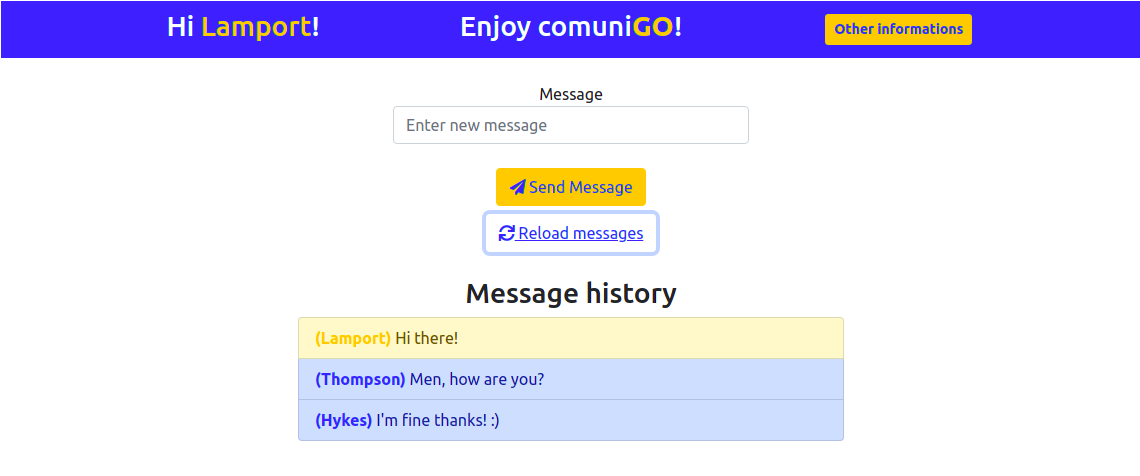
\includegraphics[width=0.4\textwidth]{figs/home.png}}
\caption{Home page di comuniGO}
\label{fig:home}
\end{figure}

L'applicazione soddisfa i requisiti richiesti dalla traccia, ovvero:
\begin{itemize}
\item prevede un servizio di registrazione per i peer che vogliono partecipare al gruppo di multicast, assumendo che la membership sia statica durante l'esecuzione;

\item prevede il supporto dei seguenti algoritmi:
\begin{enumerate}
\item multicast totalmente ordinato implementato in modo centralizzato tramite un \textsl{sequencer};

\item multicast totalmente ordinato implementato in modo decentralizzato tramite l'uso di \textsl{clock logici
scalari};

\item multicast causalmente ordinato implementato in modo decentralizzato tramite l'uso di \textsl{clock
logici vettoriali}.
\end{enumerate}
\end{itemize}

Inoltre, come richiesto dalla specifica, è stato testato il funzionamento degli algoritmi implementati nel caso in cui:
\begin{itemize}
\item vi sia un solo processo che invia il messaggio di multicast
\item molteplici processi contemporaneamente inviino un
messaggio di multicast;
\end{itemize}
e per simulare condizioni di maggiore stress nel testing è stato incluso, come consigliato, un parametro \textit{delay} configurabile che permette di specificare un ritardo nell'invio generato in modo random in un intervallo predefinito.

Per facilitare il debugging dell'applicazione, come suggerito dalla traccia,  stato implementato un flag di tipo \textit{verbose} che, se attivo, abilita la stampa di informazioni di logging con i dettagli dei messaggi inviati e ricevuti.

\section{Tecnologie adottate}
Per lo sviluppo del progetto si è fatto uso delle seguenti tecnologie:
\begin{itemize}
\item \textbf{Docker} per il supporto alla virtualizzazione;
\item \textbf{Docker compose} per coordinare l'esecuzione dei container sul singolo nodo (e.g. startup, shutdown, interconnessione degli elementi);
\item \textbf{Go} come unico linguaggio per lo sviluppo della logica applicativa;
\item \textbf{gRPC} come framework RPC per lo scambio dei messaggi fra i componenti dell'applicazione;
\item \textbf{Redis} come datastore in memory per la memorizzazione dei messaggi \textit{consegnati a livello applicativo} dai vari algoritmi;
\item \textbf{HTML}, \textbf{Javascript} (\textbf{jQuery}) e \textbf{CSS} per la realizzazione del frontend Web con cui interagire con l'applicazione.
\end{itemize}

\section{Descrizione dell'architettura}
\begin{figure}[htbp]
\centerline{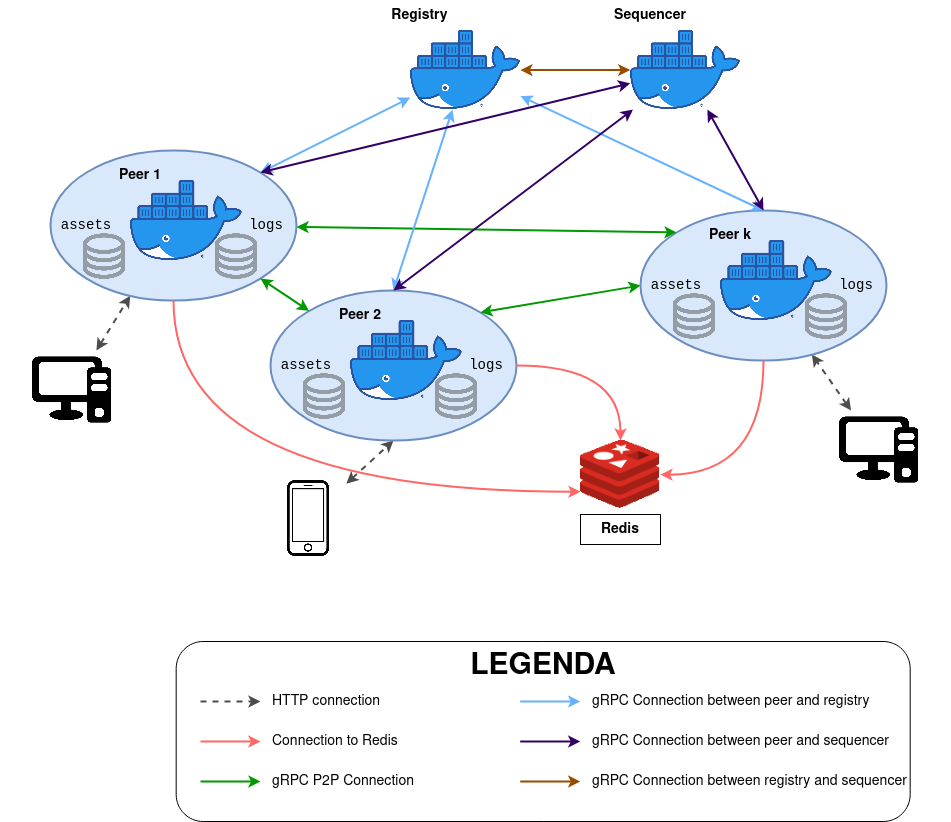
\includegraphics[width=0.4\textwidth]{figs/architecture.png}}
\caption{Architettura realizzata.}
\label{fig:architecture}
\end{figure}

In figura \ref{fig:architecture} è riportata una schematizzazione dell'architettura adottata per lo sviluppo dell'applicazione, in cui è possibile notare come:
\begin{itemize}
\item peer, servizio di registrazione e sequencer siano ciascuno incapsulato all'interno di un container differente;
\item a ciascun peer sono associati due volumi, uno per permettere che l'attività di logging sia persistente e l'altro per accedere agli assets web

\item ogni peer è connesso ad un'istanza unica di Redis al fine di consegnare e prelevare i messaggi;

\item la logica applicativa è interamente realizzata sfruttando il meccanismo RPC per qualunque coppia di endpoint;

\item l'utente finale può scambiare i propri messaggi con gli altri connessi al gruppo di multicast semplicemente utilizzando il proprio browser (o in alternativa sfruttando programmi come cURL). 
\end{itemize}
\section{Scelte progettuali}
Di seguito è riportata una carrellata di scelte effettuate nello sviluppo della soluzione proposta.

\subsection{Uso di un frontend web per l'interazione con i peer}
Per permettere l'interazione con i peer è stato scelto di realizzare un webserver implementato in Go sfruttando la libreria \texttt{labstack/echo}.

Le route servite sono di seguito analizzate brevemente:
\begin{itemize}
\item \texttt{[GET] /:} permette di accedere al portale di comunicazione effettivo, previa registrazione;
\item \texttt{[GET] /list:} permette di ottenere la lista dei messaggi ricevuti in formato json;
\item \texttt{[GET] /info:} permette di effettuare il retrieve delle informazioni necessarie a popolare l'homepage del sito;
\item \texttt{[POST] /send:} permette di inviare un messaggio, specificando come parametro:
\begin{itemize}
\item \texttt{message}: il corpo del messaggio,
\item \texttt{delay}: l'intervallo entro cui estrarre il ritardo con cui inviare il messaggio nel formato \texttt{start:end} \textbf{da usare solo in fase di test};
\end{itemize}
\item \texttt{[POST] /sign:} permette di inviare il proprio username al servizio di registrazione, specificandolo come parametro (\texttt{username}).
\end{itemize}

Le risorse statiche, ovvero i file \texttt{*.html} e \texttt{*.js}, poiché non soggetti ad alcun processo di compilazione, sono state inserite all'interno del filesystem del container come volume \textit{readonly} (\texttt{assets}). Ciò permette di:
\begin{itemize}
\item diminuire il footprint delle immagini docker prodotte
\item evitare di avviare la build dell'immagine del peer a seguito del cambiamento di alcuni elementi puramente grafici dell'applicazione
\end{itemize}

\subsection{Uso di volumi per l'attività di logging}
È stato scelto di adottare dei volumi docker per rendere l'attività di log persistente così da non dover avere il vincolo di lanciare i vari container in modalità \textit{attached}.

La tipologia di volume adottato è \textit{bind} per cui l'engine di docker non fa altro che montare la directory del filesystem locale \texttt{\$COMUNIGO\_PATH/logs} su \texttt{/logs} all'interno del container.

Per quanto riguarda l'attività di log svolta dal webserver, il formato configurato per ciascuna riga del file è il seguente:

\centerline{\scriptsize\texttt{[<time>]: method=<method>, uri=<uri>, status=<status>}}

\subsection{Uso di redis per la memorizzazione dei messaggi}
Poiché si utilizza un frontend web per interagire con l'applicazione è possibile che l'utenti aggiorni la pagina o semplicemente chiuda la tab del browser per poi riaprirla in un secondo momento.

In questo scenario per \textit{consegnare i messaggi al livello applicativo} non è sufficiente unicamente restituirli (e.g. classica stampa su terminale) perché altrimenti non si avrebbe la possibilità di ripetere l'esecuzione.

È necessario dunque memorizzarli e, al fine di disaccoppiare la logica applicativa dall'effettiva memorizzazione dei messaggi, è stato scelto di utilizzare un datastore separato.

La scelta è ricaduta su redis per diversi motivi:
\begin{itemize}
\item si integra in maniera ottimale con Go, infatti l'API mappa praticamente 1:1 con gli effettivi comandi nativi di Redis;
\item essendo la membership statica non è previsto che i peer vengano spenti ed in seguito riaccesi per partecipare sempre allo stesso gruppo per cui la natura \textit{in-memory} di Redis non rappresenta un'ostacolo;
\item le funzionalità \texttt{RPUSH} e \texttt{LRANGE} nativamente permettono di coprire il meccanismo di salvataggio e recupero dei messaggi
\end{itemize}

\subsection{Altre scelte}
\begin{itemize}
\item Nella stesura del codice è stato adottato un approccio object oriented seppure Go non è un linguaggio puramente OO come ad esempio lo è Java.

Tuttavia questo approccio ha reso possibile la stesura di un codice modulare, facilmente manutenibile ed estendibile.

\item Per l'invio dei messaggi è stato scelto di adottare connessioni TCP persistenti così da avere:
\begin{itemize}
\item un overhead inferiore in termini di messaggi di handshaking inviati;
\item la garanzia di consegna FIFO ordered dei messaggi.
\end{itemize}

\item Nel codice si è fatto massivamente uso di go routines, per parallelizzare l'esecuzione avendo un guadagno sulle prestazioni, e di canali al fine di:
\begin{itemize}
\item Permettere lo scambio di informazioni fra le varie goroutines
\item Sincronizzare le goroutines limitando l'uso esplicito di lock
\end{itemize}

\item Per implementare un meccanismo di chiusura \textit{pulita} dell'applicazione è stato utilizzato il meccanismo nativo di go dei \textit{contesti con cancellazione} in combinazione con la cattura dei segnali di \texttt{SIGINT} e \texttt{SIGTERM} che, stando alla documentazione Docker, vengono invati da docker-compose nel momento in cui si richiede lo stop dei container
\end{itemize}

\section{Descrizione dell'implementazione}
\subsection{Registrazione}
Lato frontend, la registrazione prevede che:
\begin{enumerate}
\item l'utente si colleghi ad uno dei peer del gruppo, i quali possono essere individuati tramite lo script di discovery o il programma Go apposito, descritti all'interno del README file;
\item inserisca un nome utente unico all'interno del gruppo;
\item attenda che tutti quanti i membri siano realmente connessi prima di entrare effettivamente nel portale di comunicazione.
\end{enumerate}

Lato backend invece:
\begin{enumerate}
\item il peer inoltra al servizio di registrazione l'username ricevuto dal frontend;
\item le procedure remote server-side inviano quanto ricevuto dai peer ad un'apposita go routine che mantiene la lista non ancora completa degli utenti connessi;
\item nel momento in cui si raggiunge la taglia del gruppo prevista, la routine in questione \textit{sblocca} le procedure in attesa di poter inviare la composizione del gruppo al peer richiedente
\item una volta ricevuto l'elendo dei peer connessi, esso viene inoltrato via HTTP al client web affichè:
\begin{itemize}
\item Si effettui il redirect verso il reale portale per la comunicazione
\item Si mostri un messaggio d'errore ove necessario
\end{itemize}
\end{enumerate}

\subsection{Comunicazione tramite sequencer}
Nel caso in cui la modalità di comunicazione selezionata è quella basata sull'utilizzo di un sequencer, il nodo di registrazione comunica la composizione del gruppo di multicast anche a quest'ultimo prima di terminare la sua esecuzione.

Una volta completata la fase di registrazione, la comunicazione tramite sequencer si basa sull'iter di seguito riportato:

\begin{itemize}
\item Nella comunicazione \textsl{dal peer al sequencer}
\begin{enumerate}
\item il peer inoltra al sequencer il messaggio ricevuto dal frontend; 
\item le procedure remote server-side inviano quanto ricevuto dai peer ad un'apposita goroutine responsabile di ordinare in modo univoco i messaggi ricevuti e marcarli con un apposito timestamp (\textit{sequence number})
\end{enumerate}

\item Nella comunicazione \textsl{dal sequencer al peer} ogni qual volta la go routine dedicata all'ordinamento marca un nuovo messaggio con un determinato timestamp, questo viene inoltrato sulle varie connessioni aperte in precedenza verso tutti i peer
\end{itemize}

\subsection{Comunicazione basata su clock logici scalari}
Nel caso in cui la modalità di comunicazione selezionata è quella basata sull'utilizzo del clock logico scalare, una volta completata la fase di registrazione, la comunicazione si basa sull'approccio di seguito descritto:

\begin{itemize}
\item per l'\textsl{invio degli update} una goroutine ad hoc preleva quanto inserito dall'utente come corpo del messaggio, appone ad esso il proprio timestamp incrementato di una unità e lo inoltra sulle varie connessioni in precedenza aperte verso i restanti partecipanti al gruppo di multicast;

\item alla \textsl{ricezione degli update}:
\begin{enumerate}
\item si aggiorna il clock, ponendolo pari a:
\begin{equation}
L = \max\lbrace L, t \rbrace
\end{equation}
dove $L$ è il clock logico scalare locale del peer e $t$ quello contenuto nel messaggio ricevuto;
\item si riscontra la ricezione inviando un ack a tutti i partecipanti del gruppo;
\item si inserisce il messaggio all'interno della coda dei messaggi pendenti e la si ordina rispetto al clock logico scalare e l'identificativo del membro (\texttt{username});
\item si consegnano i messaggi per cui valgono le seguenti condizioni:
\begin{itemize}
\item sono i primi nella coda totalmente ordinata;
\item sono stati riscontrati da tutti gli altri membri;
\item per ogni altro membro sono presenti messaggi in coda.
\end{itemize}
\end{enumerate}

\item Alla \textsl{ricezione degli ack}:
\begin{enumerate}
\item si incrementa il contatore degli ack associato al messaggio riscontrato;
\item si consegnano i messaggi per cui vale la condizione sopra proposta.
\end{enumerate}
\end{itemize}

Essendo questo algoritmo indubbiamente il più elaborato fra i tre, di seguito è riportata un analisi sintetica delle strutture dati utilizzate per renderlo quanto più possibile efficiente.
\begin{itemize}
\item Viene utilizzato uno slice nativo di Go per la memorizzazione dei messaggi pendenti, il che implica un costo $O(n)$ ad ogni nuovo inserimento, per via della necessità di mantenere l'ordinamento.

\item Viene utilizzata una mappa stringa $\to$ intero per contare gli ack ricevuti per ciascun messaggio pendente affinché il costo dell'incremento sia $O(1)$.

È opportuno osservare che mantenere il contatore degli ack come metadato presente all'interno di ogni entry della lista dei messaggi avrebbe causato un costo per l'aggioramento, nel caso peggiore, pari a $O(n)$ per via della ricerca sequenziale, dove $n$ è pari alla taglia della coda.

\item Viene utilizzata una mappa stringa $\to$ intero per tener traccia del numero di pacchetti in coda presenti per ciascun peer connesso al gruppo di multicast.

Questa soluzione permette di realizzare la condizione \textit{``per ogni altro membro sono presenti messaggi in coda"} con un costo $O(k)$, dove $k$ è pari al numero di peer connessi ($k-1$ accessi alla mappa ciascuno dei quali a costo $O(1)$).

È opportuno osservare che nel caso in cui non fosse stata utilizzata questa struttura dati, il costo della verifica sarebbe stato pari a $O(n)$, dove $n$ è pari al numero di messaggi in coda.

Ovviamente in scenari reali d'utilizzo $k << n$.
\end{itemize}

\subsection{Comunicazione basata su clock logici vettoriali}
Nel caso in cui la modalità di comunicazione selezionata è quella basata sull'utilizzo del clock logico vettoriale, una volta completata la fase di registrazione, la comunicazione si basa sull'approccio di seguito descritto:
\begin{itemize}
\item per l'\textsl{invio dei messaggi} da parte del peer $i$-esimo, una goroutine ad hoc:
\begin{itemize}
\item preleva quanto inserito dall'utente come corpo del messaggio;
\item appone ad esso il proprio timestamp dopo averlo modificato come segue:
\begin{equation}
V_i[i] = V_i[i] + 1
\end{equation}
\item inoltra il messaggio sulle varie connessioni in precedenza aperte verso i restanti partecipanti al gruppo di multicast
\item consegna direttamente il messaggio poiché certamente rispetta la causalità
\end{itemize}

\item alla \textsl{ricezione di un messaggio} proveniente dal peer $i$-esimo da parte del peer $j$-esimo :
\begin{enumerate}
\item si inserisce il messaggio all'interno della coda dei messaggi pendenti;
\item si consegnano tutti i messaggi per cui valgono le seguenti condizioni:
\begin{itemize}
\item $t[i] = V_j[i] + 1$
\item $t[k] \leq V_j[k]$ per ogni $k\neq i$
\end{itemize}
\end{enumerate}
\end{itemize}

\section{Testing \& debugging}
Per lo sviluppo dei casi di test si è fatto uso del supporto \textit{built-in} offerto da Go, ovvero \texttt{go test}.

Nel caso di \textsl{invio singolo adottando multicast totalmente ordinato} è stato simulato l'evento di send per ciascun processo connesso, attendendo tra un invio ed il successivo un tempo pari al massimo delay sperimentabile così da avere la garanzia che tutti i messaggi ricevano la medesima sequenza ordinata di messaggi

Nel caso di \textsl{invio multiplo adottando multicast totalmente ordinato} è stato realizzato uno scenario analogo ove tuttavia anziché inviare l'uno dopo l'altro i processi mandano i propri messaggi in modo simultaneo mediante l'ausilio di go,routines

Una volta effettuato l'invio, in entrambi i casi i processi effettuano il retrieve della lista dei messaggi consegnati per poi:
\begin{itemize}
\item nel caso di implmentazione tramite \textsl{sequencer} verificare che le liste ricevute siano tutte uguali;
\item nel caso di implementazione tramite \textsl{clock logico scalare} verificare che la parte comune a tutte le liste sia uguale.

Questo perché per via del meccanismo di consegna è possibile ad esempio si verifichi che:
\begin{itemize}
\item il processo $A$ riceva $k$ messaggi;
\item il processo $B$ riceva $h$ messaggi;
\item il processo $C$ riceva $l$ messaggi
\end{itemize}
con $l\leq h\leq k$. In questo scenario il test verifica che i primi $l$ messaggi di ciascuna lista siano equivalenti
\end{itemize}


Per il testing dell'algoritmo basato sull'utilizzo dei clock logici vettoriali è stato scelto di verificare l'effettivo rispetto della causalità nel modo seguente:
\begin{enumerate}
\item ciascun peer invia un messaggio avente come body il proprio username;
\item attende un certo $\Delta t$;
\item effettua il retrieve dei messaggi ricevuti;
\item costruisce un messaggio \textit{riassuntivo} contenente l'elenco dei body ricevuti separati da \texttt{":"} (e.g \texttt{"A:B"});
\item invia il messaggio riassuntivo,
\item si verifica per ciascun peer che all'interno della lista dei messaggi quelli \textit{riassuntivi} sono successivi a quelli che riscontrano.

Ad esempio se il messaggio riassuntivo è \texttt{"A:B"} si verifica che i messaggi \texttt{"A"} e \texttt{"B"} lo precedano in ogni lista
\end{enumerate}

Ovviamente ciò che differenzia il caso di test di invio singolo da quello di invio multiplo è la modalità di invio dei messaggi da parte dei peer:
\begin{itemize}
\item Nel caso \textsl{singolo} se ne invia uno alla volta
\item Nel caso \textsl{multiplo} si fa uso di go routines per simulare il parallelismo
\end{itemize}

Per quanto riguarda il debugging, poiché l'attività di logging è stata resa persistente e quindi è possibile ispezionare nel dettaglio come agiscono i peer, è stato scelto di implementare la logica collegata al flag \texttt{verbose} semplicemente mostrando su console javascript il detaglio dei messaggi ricecvuti comprensivo di timestamp associato ad essi, come mostrato in figura \ref{fig:debug}

\begin{figure}[htbp]
\centerline{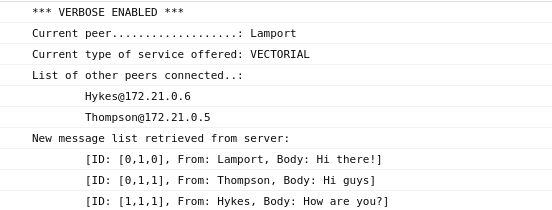
\includegraphics[width=0.4\textwidth]{figs/debug.png}}
\caption{Implementazione del flag \texttt{verbose}}
\label{fig:debug}
\end{figure}

\section{Modifiche necessario per il deployment su cluster reali}
Nel momento in cui si volesse deployare questa applicazione distribuita su un cluster di nodi (e.g. mediante l'ausilio di Kubernetes o di istanze EC2) ovviamente non sarebbe idoneo utilizzare un unica istanza attiva di Redis poiché si perderebbe il vantaggio della decentralizzazione degli algoritmi tornando ad avere un SPOF.

Lo scenario ideale di deployment sarebbe dunque quello in cui su ciascun nodo fosse presente un istanza di peer e una di redis, avendo dunque un'architettura come quella riportata in figura \ref{fig:architecture-real}.

Avere la configurazione dei peer non hardcoded all'interno del sorgente, bensì facilmente modificabile tramite:
\begin{itemize}
\item il file \texttt{\$COMUNIGO\_PATH/build/comunigo.cfg};
\item i parametri passati da linea di comando allo script di startup
\end{itemize}
permette di realizzare il porting a quest'architettura più realistica in modo semplice senza che sia necessario modificare in modo massivo il codice.

\begin{figure}[htbp]
\centerline{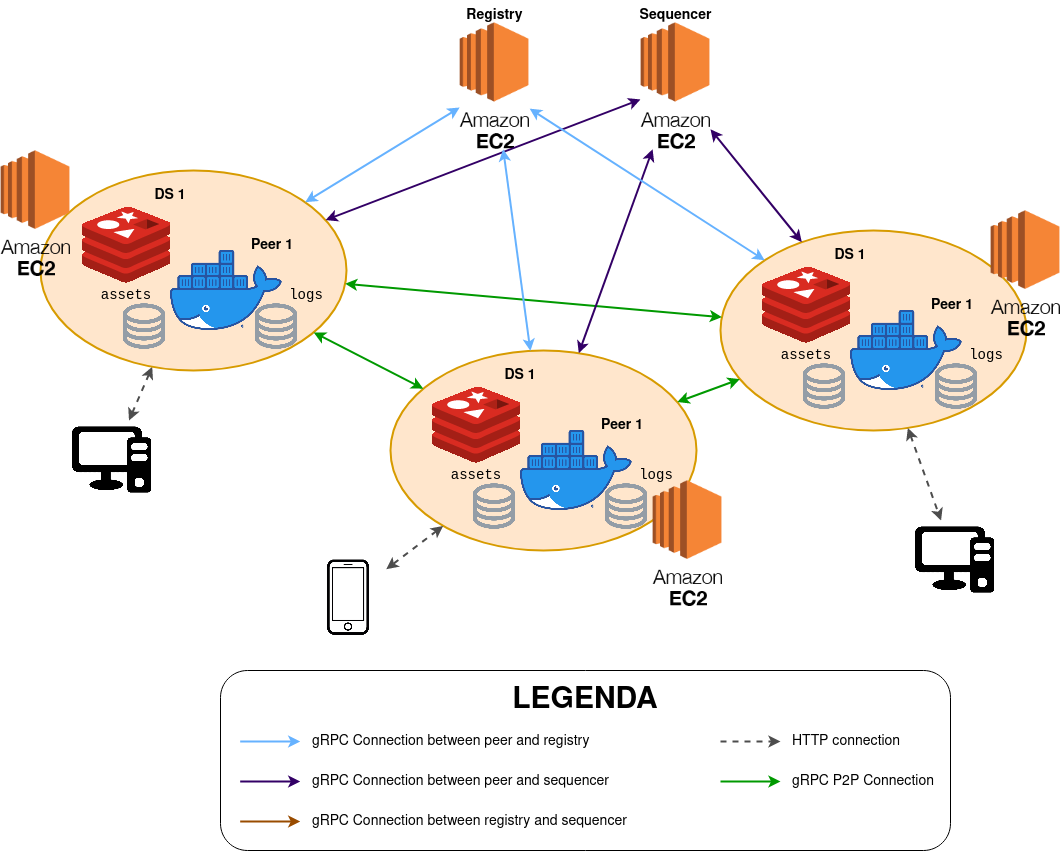
\includegraphics[width=0.4\textwidth]{figs/architecture-real.png}}
\caption{Possibile architettura su deployment reale}
\label{fig:architecture-real}
\end{figure}

\end{document}
